% THIS IS SIGPROC-SP.TEX - VERSION 3.1
% WORKS WITH V3.2SP OF ACM_PROC_ARTICLE-SP.CLS
% APRIL 2009
%
% It is an example file showing how to use the 'acm_proc_article-sp.cls' V3.2SP
% LaTeX2e document class file for Conference Proceedings submissions.
% ----------------------------------------------------------------------------------------------------------------
% This .tex file (and associated .cls V3.2SP) *DOES NOT* produce:
%       1) The Permission Statement
%       2) The Conference (location) Info information
%       3) The Copyright Line with ACM data
%       4) Page numbering
% ---------------------------------------------------------------------------------------------------------------
% It is an example which *does* use the .bib file (from which the .bbl file
% is produced).
% REMEMBER HOWEVER: After having produced the .bbl file,
% and prior to final submission,
% you need to 'insert'  your .bbl file into your source .tex file so as to provide
% ONE 'self-contained' source file.
%
% Questions regarding SIGS should be sent to
% Adrienne Griscti ---> griscti@acm.org
%
% Questions/suggestions regarding the guidelines, .tex and .cls files, etc. to
% Gerald Murray ---> murray@hq.acm.org
%
% For tracking purposes - this is V3.1SP - APRIL 2009

\documentclass{acm_proc_article-sp}
\usepackage{float}

\begin{document}

\raggedbottom

\title{Distributed Histogram Creation with MapReduce and MPI}
\subtitle{CSC 569}

\numberofauthors{4} 
\author{
\alignauthor
Ian Dunn\\
       \affaddr{Computer Science Department}\\
       \affaddr{Cal Poly}\\
       \affaddr{San Luis Obispo, California}\\
       \email{idunn01@calpoly.edu}
\alignauthor
Toshi Kuboi\\
       \affaddr{Computer Science Department}\\
       \affaddr{Cal Poly}\\
       \affaddr{San Luis Obispo, California}\\
       \email{tkuboi@calpoly.edu}
       \and % go to new row
\alignauthor
Mitchell Rosen\\
       \affaddr{Computer Science Department}\\
       \affaddr{Cal Poly}\\
       \affaddr{San Luis Obispo, California}\\
       \email{mwrosen@calpoly.edu}
\alignauthor
Austin Wylie\\
       \affaddr{Computer Science Department}\\
       \affaddr{Cal Poly}\\
       \affaddr{San Luis Obispo, California}\\
       \email{awylie@calpoly.edu}
}

\date{30 October 2013}

\maketitle

\section{Introduction}
This project familiarized us with MapReduce, MPI, and distributed computing performance tradeoffs by calculating vector sums and histograms on a cluster of five Raspberry Pis. We wrote two programs that, given a pair of input files containing vectors of floating-point numbers, summed those vectors and created histograms for each of them as well as the vector sum.

One program's aim was to distribute the work among the five Pis and compute the results as quickly as possible. The other program made this process fault-tolerant (albeit less efficient) with a different method that allowed one node to be disconnected during its run.

\section{Part A: Distributed Performance}
This section describes our non-fault-tolerant programs that distributes histogram creation among the five nodes.

\subsection{Program Setup}
\subsubsection{MR-MPI}
Using MPI, this first MR-MPI-based program sends the input vector files residing on the master to the other four nodes as character arrays. Each node then breaks the input vector character arrays into large chunks and maps them.

The map callback tokenizes each large string on whitespace, converts each token into a float, and creates KeyValues with the float's index as the key and the float as the value. The addition happens after the two vectors' MapReduce objects are combined (with MapReduce's add and collate functions), and the results are reduced by summing the values for each index and creating new KeyValues with the index as key and the summed result as value.

Now that each of the three vectors (the third being the summed vector) are available, each one's maximum is found by performing a built-in MapReduce sort on the values and returning the first element of the vector.

Next, histogram counts are calculated with a map function that creates KeyValues with a bin number as key, a collate that combines them, and a reduce that counts the number of (empty or null) values per bin number. Those counts are then scanned into arrays on the master node, and are written to result files (in addition to the summed vector).

\subsubsection{MPI}
We ran into an issue where our MR-MPI setup wouldn't calculate histograms for input vector sizes 10,000, 100,000, or 10,000,000, so we added another implementation based solely on MPI (without MapReduce) that performs the same task.

This version of the program has the master break the input vectors into equal-sized chunks and send them to slaves, which convert their two vector portions into floats and sum them. The slaves then return those sums to the master, which creates the histogram.

\clearpage

\subsection{Performance Analysis}
This section includes the performance information for our three implementations as well as the outputted program results (shown in Figures~\ref{hist10000} through~\ref{hist10000000c}).

\subsubsection{MR-MPI}
The MR-MPI implementation runtimes are shown in Table~\ref{MrMPITable} and Figure~\ref{MrMPI}.

\begin{table}[tbp]
\centering
\caption{MR-MPI Histogram Creation Performance}
\label{MrMPITable}
\begin{tabular}{ c || c }
	Input Size & Time (s) \\ \hline
    10 & 2.157 \\
    1,000,000 & 95.231 \\
\end{tabular}
\end{table}

\begin{figure*}[tbp]
  \centering
  \caption{Performance with MR-MPI}
	\label{MrMPI}
  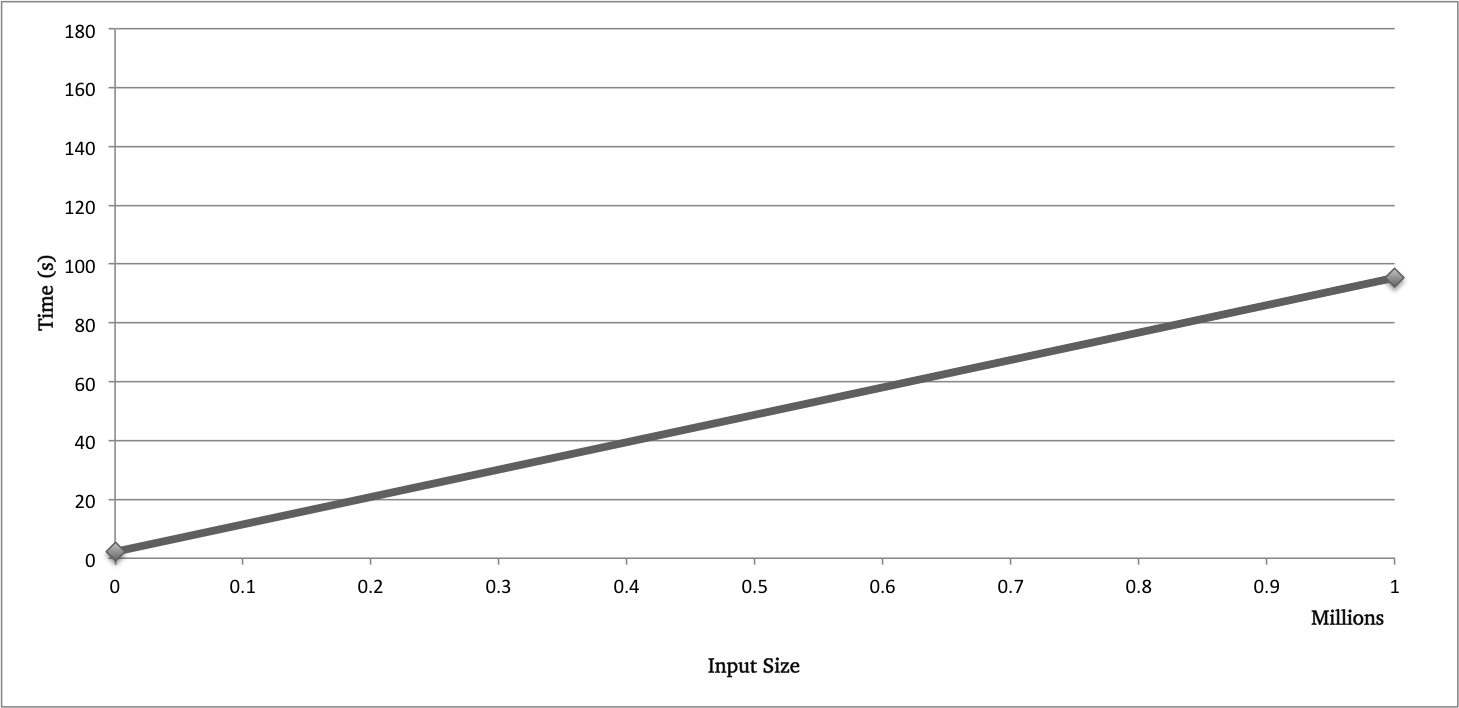
\includegraphics[width=40pc]{Pics/MrMPI.png}
\end{figure*}

\subsubsection{MPI}
The MPI implementation runtimes are shown in Table~\ref{MPITable} and Figure~\ref{MPI}.

\begin{table}[tbp]
\centering
\caption{MPI Histogram Creation Performance}
\label{MPITable}
\begin{tabular}{ c || c }
	Input Size & Time (s) \\ \hline
    10,000 & 1.990 \\
    100,000 & 3.525 \\
    1,000,000 & 17.494 \\
    10,000,000 & 170.553 \\
\end{tabular}
\end{table}

%%%

\begin{figure*}[tbp]
  \centering
  \caption{Performance with MPI}
	\label{MPI}
  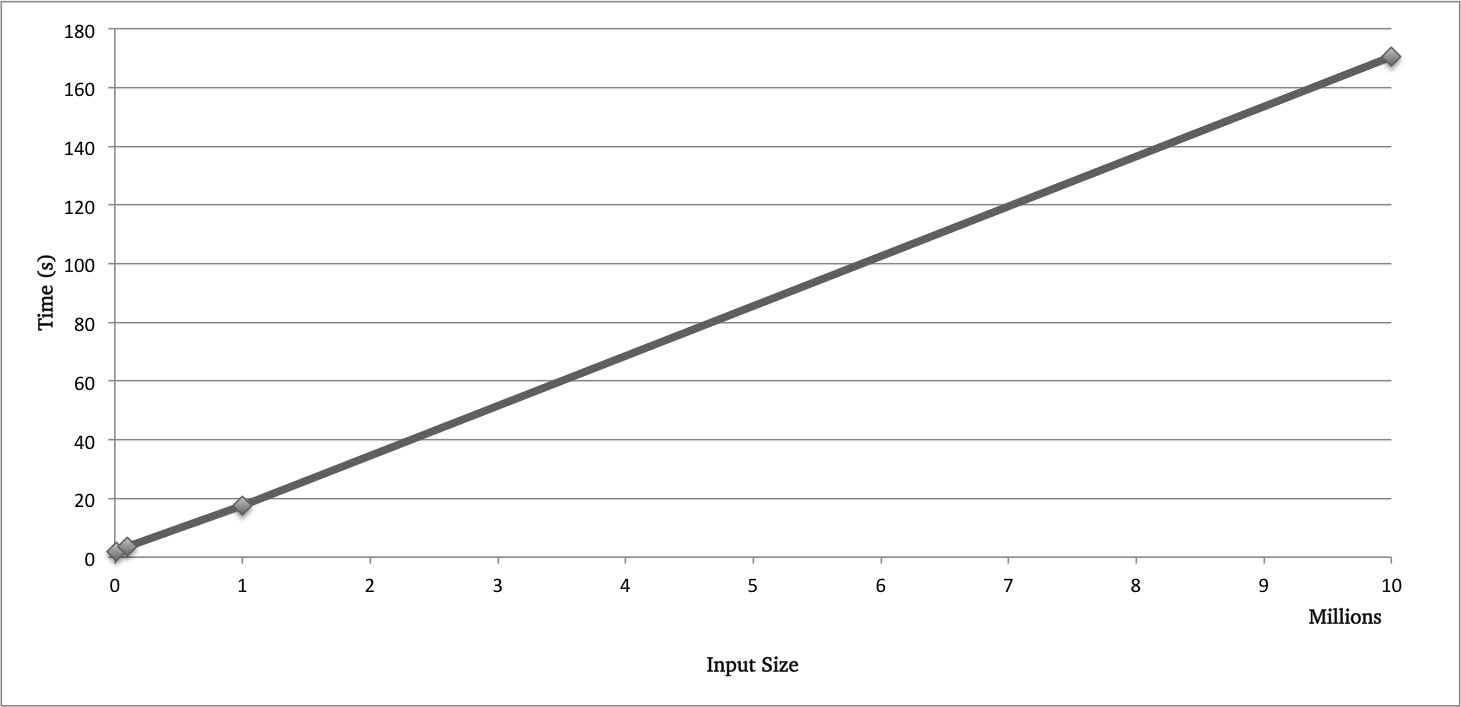
\includegraphics[width=40pc]{Pics/MPI.png}
\end{figure*}

%%%

\begin{figure*}[tbp]
  \centering
  \caption{Histogram for 10,000-Count Vectors}
	\label{hist10000}
  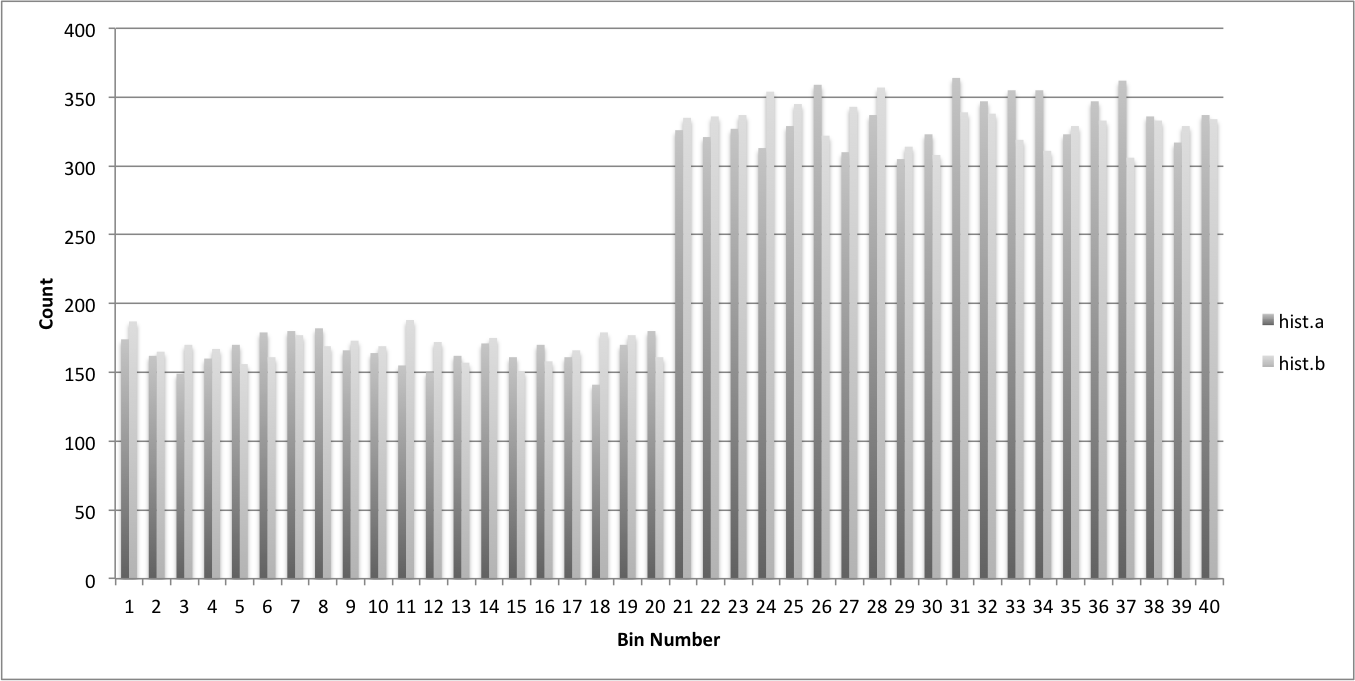
\includegraphics[width=40pc]{Pics/10000.png}
\end{figure*}

\begin{figure*}[tbp]
  \centering
  \caption{Histogram for 100,000-Count Vectors}
	\label{hist100000}
  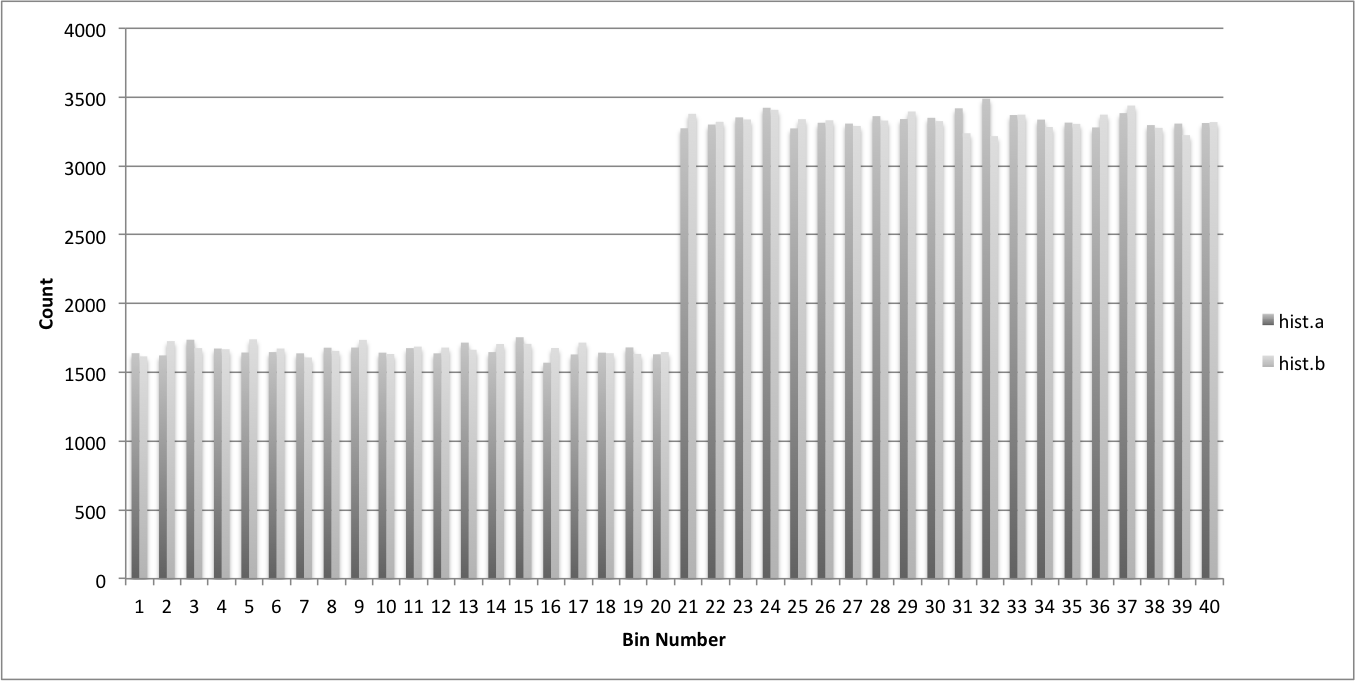
\includegraphics[width=40pc]{Pics/100000.png}
\end{figure*}

\begin{figure*}[tbp]
  \centering
  \caption{Histogram for 1,000,000-Count Vectors}
	\label{hist1000000}
  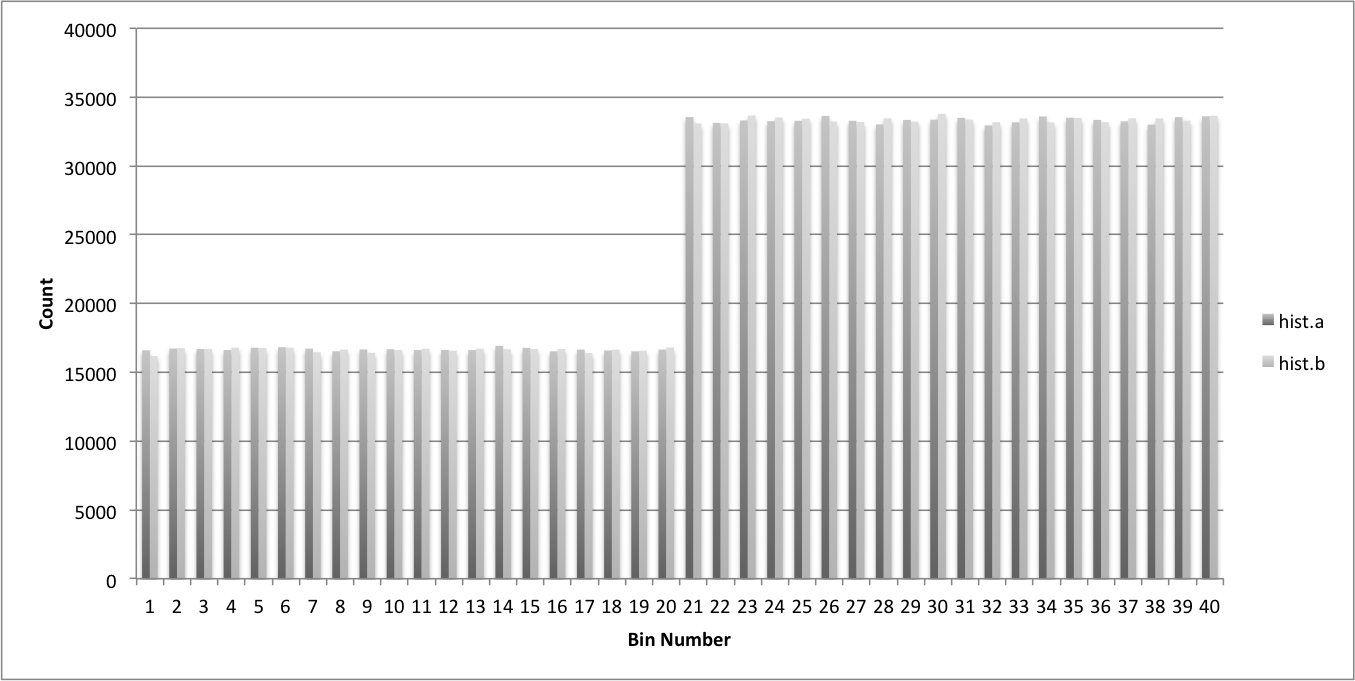
\includegraphics[width=40pc]{Pics/1000000.png}
\end{figure*}

\begin{figure*}[tbp]
  \centering
  \caption{Histogram for 10,000,000-Count Vectors}
	\label{hist10000000}
  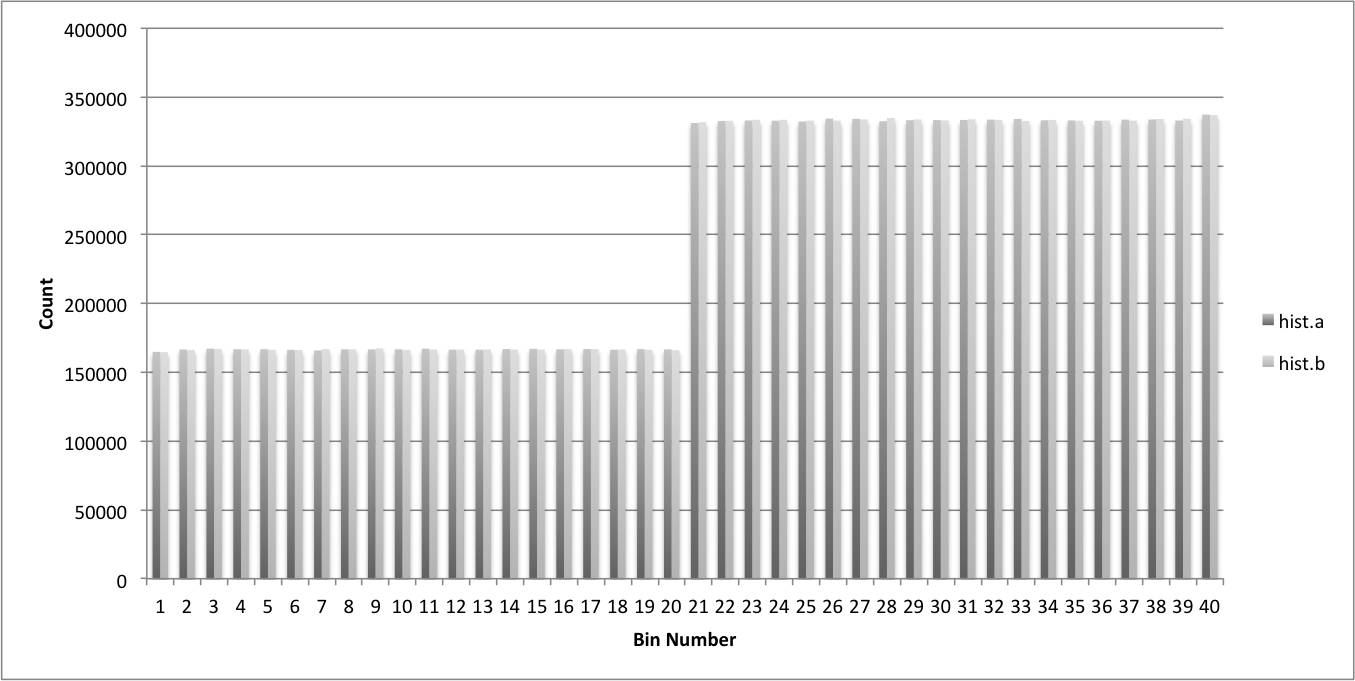
\includegraphics[width=40pc]{Pics/10000000.png}
\end{figure*}

%%%

\begin{figure*}[tbp]
  \centering
  \caption{Histogram for 10,000-Count Vector Sum}
	\label{hist10000c}
  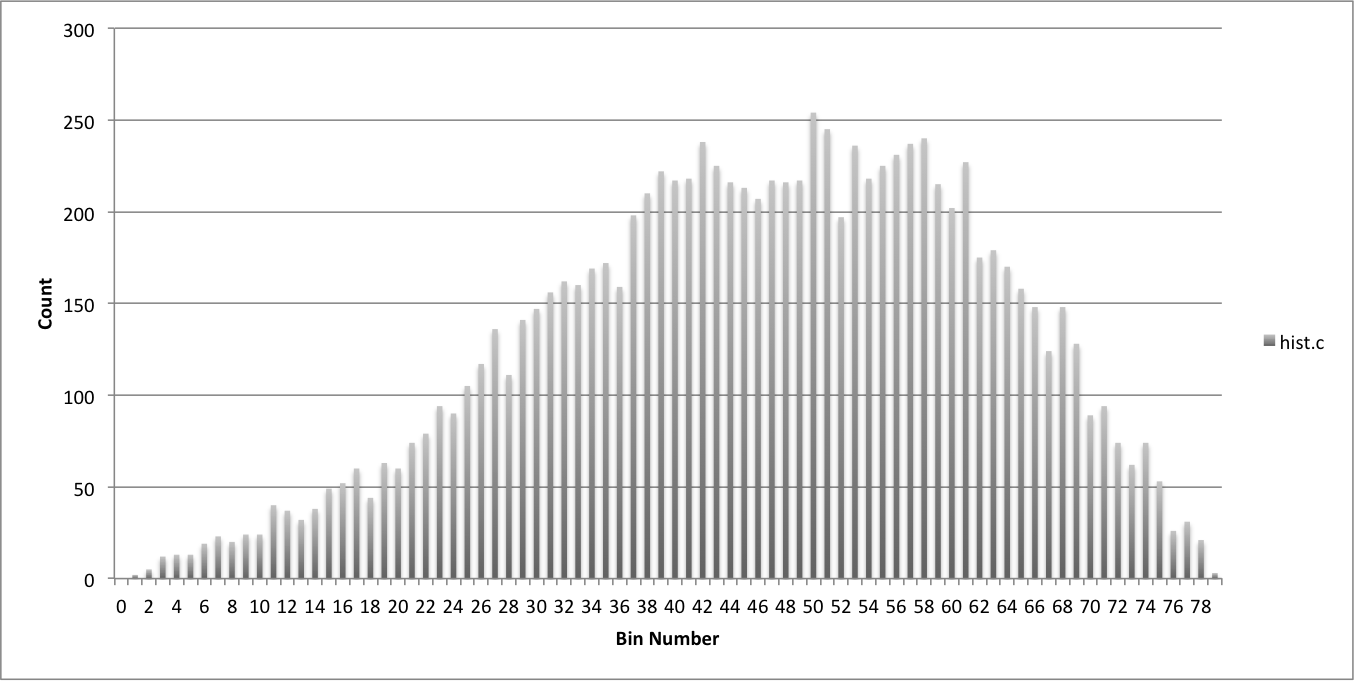
\includegraphics[width=40pc]{Pics/10000c.png}
\end{figure*}

\begin{figure*}[tbp]
  \centering
  \caption{Histogram for 100,000-Count Vector Sum}
	\label{hist100000c}
  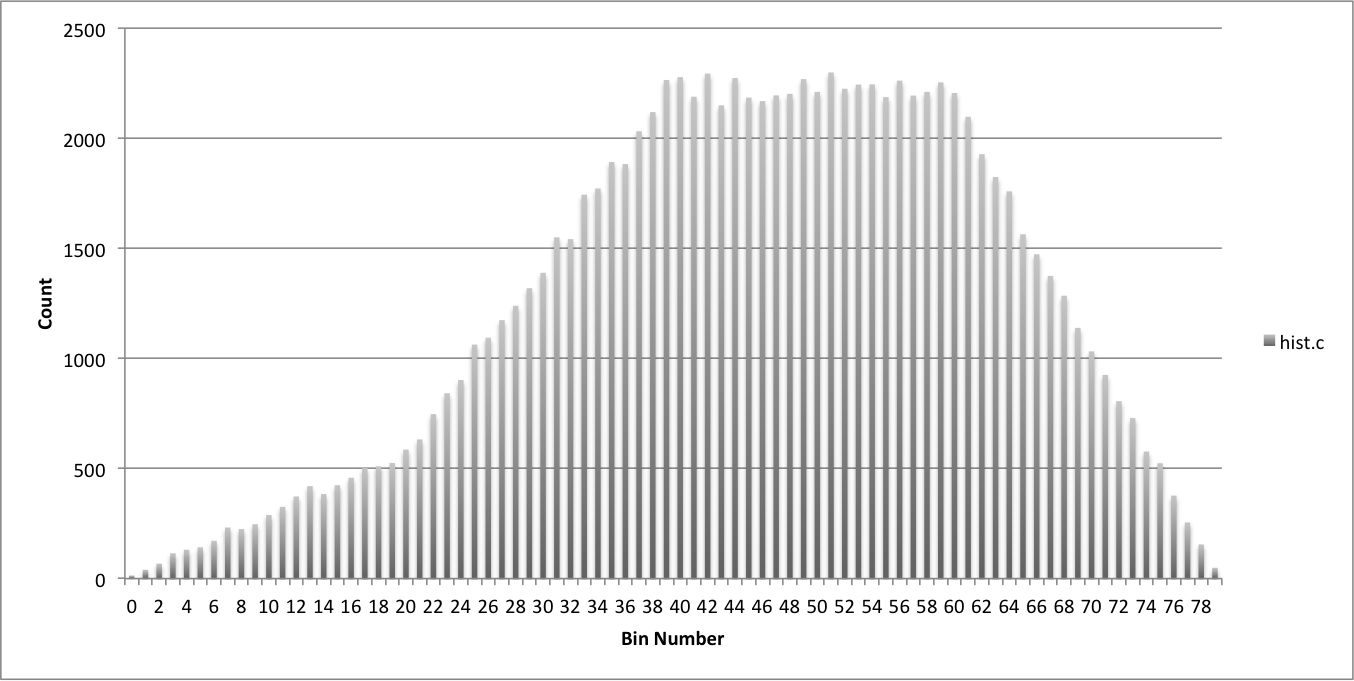
\includegraphics[width=40pc]{Pics/100000c.png}
\end{figure*}

\begin{figure*}[tbp]
  \centering
  \caption{Histogram for 1,000,000-Count Vector Sum}
	\label{hist1000000c}
  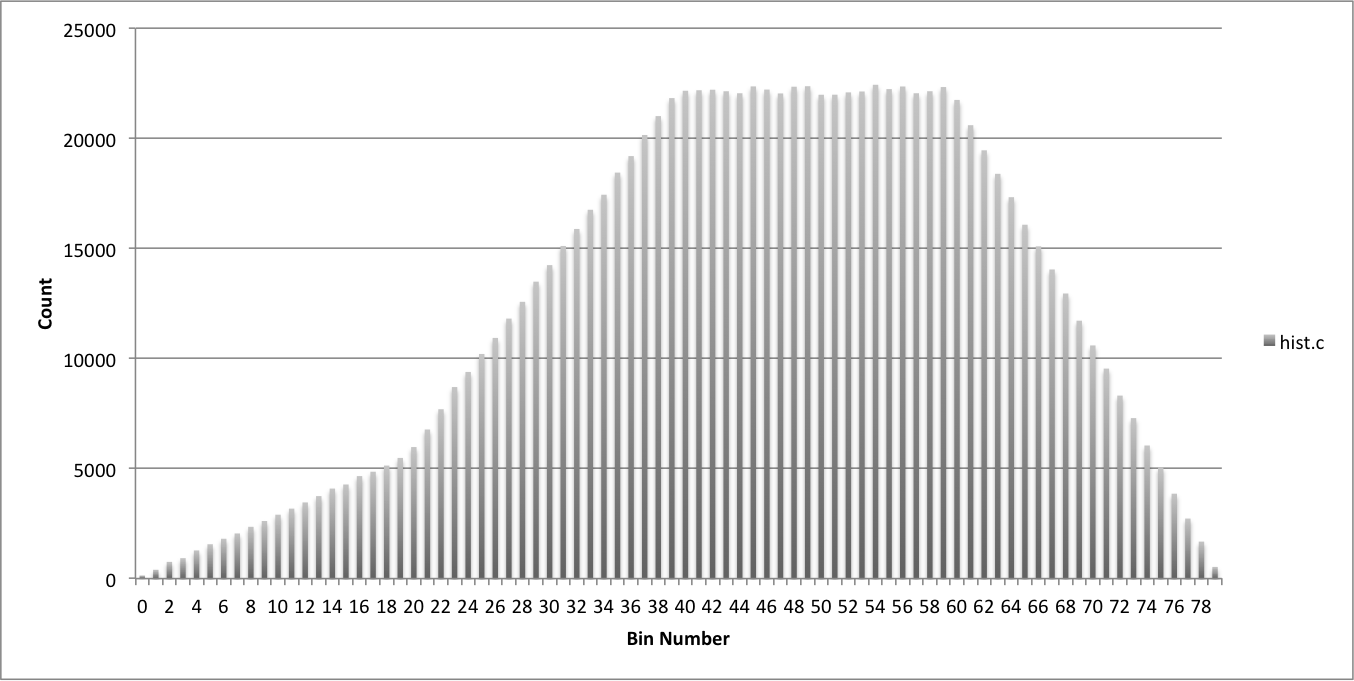
\includegraphics[width=40pc]{Pics/1000000c.png}
\end{figure*}

\begin{figure*}[tbp]
  \centering
  \caption{Histogram for 10,000,000-Count Vector Sum}
	\label{hist10000000c}
  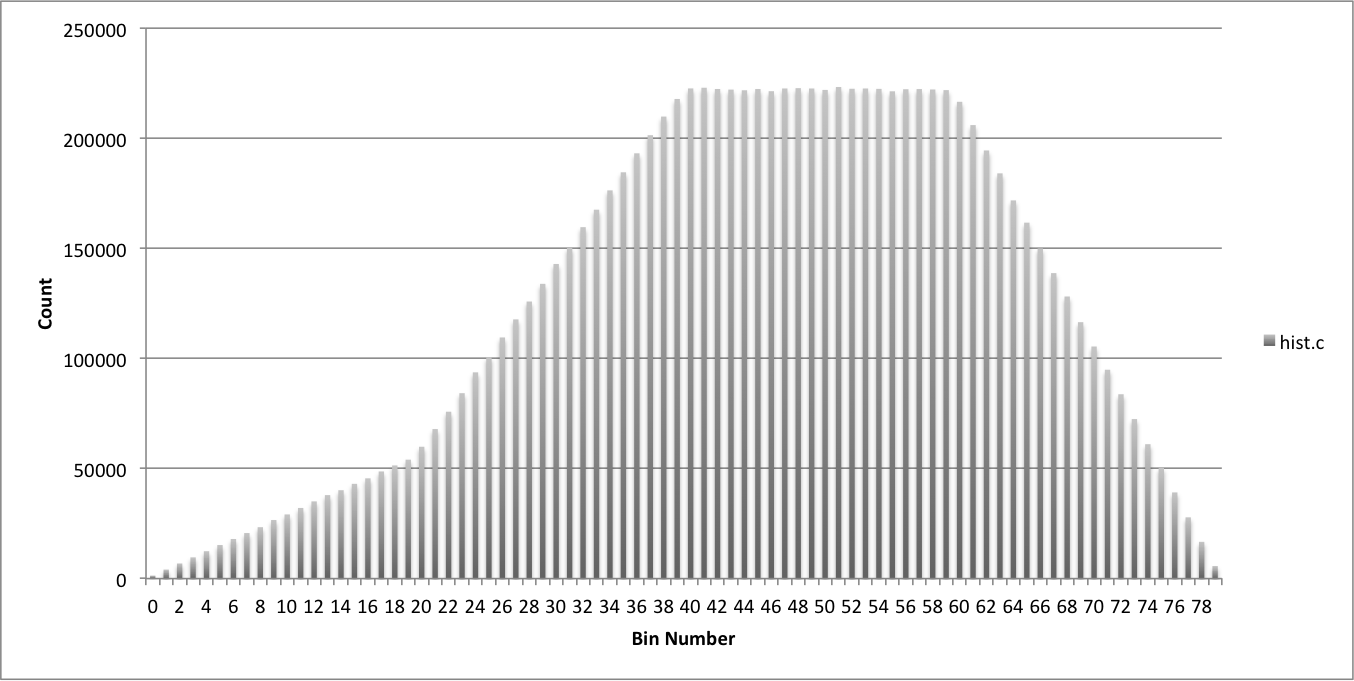
\includegraphics[width=40pc]{Pics/10000000c.png}
\end{figure*}

\section{Part B: Fault-Tolerance}
This section describes our fault-tolerant program that distributes histogram creation among the five nodes.

\subsection{Program Setup}
The fault-tolerant program using MPI first has the master read and parse the input files. The master forks one process and opens one pipe for every slave node. Each extra process sends a single pair of floats to its respective node, and the slave node adds the floats and sends back the sum. The extra process waits for the node response indefinitely and sends back the result through the pipe (if such response comes); it then calls exit(0) to avoid MPI\_Finalize.

The master computes the sum for all vector elements and waits five seconds for extra processes to catch up. This wait is performed using select() and may be interrupted by an MPI\_Recv returning. Master continually retries to wait until either the wait times equals the number of processors or the wait is successful.

The master then performs a 0.5-second select on each child's pipe to see if anything is ready to read. If a read is possible, the result is read and compared to the master's calculation. In the event of a mismatch, an error is reported and the slave's version is accepted.

Last, master sends SIGKILL to all children, makes histogram and writes output files, sends SIGKTERM to its parent, and sends SIGKILL to itself.

\subsection{Performance Analysis}
Just as a point of reference, on average, this fault-tolerant implementation could complete the 1,000,000-element test in 42 seconds (most of which is spent in file reading and writing). A node death adds approximately 0.5 seconds.

\bibliographystyle{abbrv}
%\bibliography{sample}

%\balancecolumns 

\end{document}
